\chapterimage{FutureChapterImage2.png}
\chapter{Wastewater Treatment - Future}

\section{Water Resource Recovery Facility - WRRF}\index{Water Resource Recovery Facility - WRRF}
\begin{itemize}
\item Originally, the function of a wastewater treatment plant was collection, treatment and disposal which was driven solely by the need to reduce human disease and to protect the environment.
\item It was soon realized that wastewater contains valuable elements like organic matter, phosphorus, nitrogen, rare metals and thermal energy
\item The scope of wastewater treatment has now evolved to encompass recovering valuable resources contained in the wastewater.
\item The wastewater treatment plant is now known as a water resource recovery facility (WRRF). 
\item This change reflects the new focus on the products and benefits of treatment rather than its original and only objective - treating water for sanitation.
\item The WRRF is being adapted into the concept of the circular economy in which products, materials (and raw materials) remain in the economy for as long as possible, and waste is treated as secondary raw materials that can be recycled to process and re-used.  This distinguishes it from a linear economy which is based on the: "take-make-use-dispose" system, in which waste is usually the last stage of the product life cycle.

\end{itemize}

\subsection{Water}\index{Water}
\begin{itemize}
\item Municipal wastewater reuse offers the potential to significantly increase the nation’s total available water resources. Of the 32 billion gallons of treated wastewater discharged nationally, approximately 12 billion gallons of treated wastewater is discharged each day to an ocean or estuary.
\item WRRF is key to the use of treated wastewater, or “reclaimed” water, for beneficial purposes such as drinking, irrigation, or industrial uses—is one option that has helped some communities significantly expand their water supplies.
\item Wastewater can be treated to various qualities to satisfy demand from different sectors, including industry and agriculture. It can be used to maintain the environmental flow, or even reused as drinking water. 
\item Wastewater treatment is one solution to the water scarcity issue, and also to the problem of water security, freeing water resources for other uses or for preservation.
\end{itemize}




\subsection{Energy}\index{Energy}
\begin{itemize}
\item In the US, municipal wastewater treatment plants consume 30 terawatt-hours per year of electricity which is about 0.1\% of the total electrical consumption.  
\item WRRFs have the potential to be energy neutral or even net energy producers through comprehensive energy management approaches, incorporating efficient practices, and generating renewable energy from their by-products, such as biosolids.

\item By making the treatment processes more energy efficient and through the recovery of chemical or calorific energy in the wastewater play a key role in reducing the carbon foot print of the WRRF. 

\item Given the amount of chemical or calorific energy contained in wastewater, the goal is for the WRRFs to be energy neutral or even energy positive - which is to produce same or more energy than the energy needed for treatment.
\end{itemize}


\subsection{Nutrients}\index{Nutrients}
\begin{itemize}
\item Nutrient recovery is the practice of recovering nutrients such as nitrogen and phosphorus from used water streams that would otherwise be discarded/disposed and converting them into fertilizer used for ecological and agricultural purposes. 
\item Phosphate used in fertilizers is manufactured from phosphate rock using a very environmentally detrimental mining process.  Recovery/reuse of phosphate from wastewater mitigates dependence on this mined mineral.
\end{itemize} 
Nutrient recovery at a WRRF is accomplished using one of following two methods:
\begin{enumerate}[1.] 
\item By precipitating phosphorous as struvite crystals using a dedicated reactor. The struvite crystals are collected and resold as fertilizer which has a resale value ranging from \$100-\$600 per dry ton.  Benefits of this method include:
\begin{itemize}
\item Generation of revenue from the fertilizer produced
\item Reduces fouling of equipment due to precipitation of struvite formed during the solids treatment process
\item Allows for meeting NPDES nutrients discharge limits
\end{itemize}
\item Nutrient recovery can also be achieved through the land application of biosolids. Benefits of land application of biosolids include:
\begin{itemize}
\item Provide primary nutrients - nitrogen and phosphorous and secondary nutrients such as calcium, iron, magnesium and zinc for crops.
\item The organic carbon and organic matter in the biosolids help build better soils. 
\item Allows for sequestering carbon in the soil.
\end{itemize}
\end{enumerate}


\section{Challenges to WRRF}\index{Challenges to WRRF}

\subsection{Constituents of Emerging Concern}\index{Constituents of Emerging Concern}
\begin{itemize}
\item Constituents of Emerging Concern (CECs) include a variety of substances such as medicines, personal care products, flame retardants, algal toxins, micorplastics, and many others that are not currently federally regulated but known to occur in water.
\item Some of these CECs, incuding hormones, PFAS, and endocrine disruptors are known to pose health risks to humans and aquatic life.
\item Although some CECs that reach WRRFs are destroyed through wastewater treatment and solids processing, some recalcitrant microconstituents and their metabolites may pass through the treatment process intact and may end up in the effluent or biosolids. 
\item Both, the dose (concentration) of the CEC present and frequency/duration of exposure is important for interpreting possible risk to ecological and human health.
\item The CECs move in their complex cycling through surface and groundwaters across the planet - from potable water to wastewater and viceversa as potable water is converted into wastewater followed by uptake of the treated wastewater by the potable water supply system through groundwater contaminated by the percolation of these CECs in land applied wastewater biosolids or through the CECs in the treated wastewater discharge to surface water such as a lake or river.
\item The CECs concentrations in the plant influent range typically in nano-g/L to micro-g/L , in effluent from non-detect to nano-g/L, and in biosolids the concentrations vary from micro-g/kg to mg/kg.
\end{itemize}


\subsection{Decentralized and Distributed Systems}\index{Decentralized and Distributed Systems}
\begin{itemize}
\item To make the wastewater treatment systems more sustainable and to overcome the issues of a centralized system where wastewater is collected from various areas and cities in urban areas and conveyed to a centrally located plant for treatment, it is imperative to consider 
\item \textbf{Distributed systems} are in different geographical locations, but are linked to a central system either physically, or by management. \textbf{Decentralized systems} can be located in a different geographical location, but are not linked physically, or are not managed under the umbrella of a centralized system.
\item Through the selection of correct locations and appropriate technologies, distributed or decentralized systems can:
\begin{itemize}
\item Provide environmental benefits, such as nutrient and pathogen removal
\item Provide water for direct potable reuse and non-potable water in both rural and urban settings for purposes such as flushing, cooling and heating, landscaping, and subsurface irrigation drip.
\end{itemize}
\end{itemize}


\subsection{Climate Change}\index{Climate Change} 
\begin{itemize}
\item Climate change has directly impacted water resources by altering precipitation patterns, severe drought and floods, snowpack amount, elevation, stream flow, and rising sea levels. 
\item This has created a direct need for utilities to manage local water resources to lessen the potential impact of climate change. 
\item By increasing water reuse, developing resiliency and other actions, WRRFs can be a leader in fighting and preparing for climate change effects.
\item Driven largely by climate change factors, lower carbon footprint - the amount of carbon dioxide and other carbon compounds emitted due to the consumption of fossil fuels (energy), and lower energy demands are now being factored in when assessing wastewater treatment options.
\end{itemize}
\newpage
\begin{center}
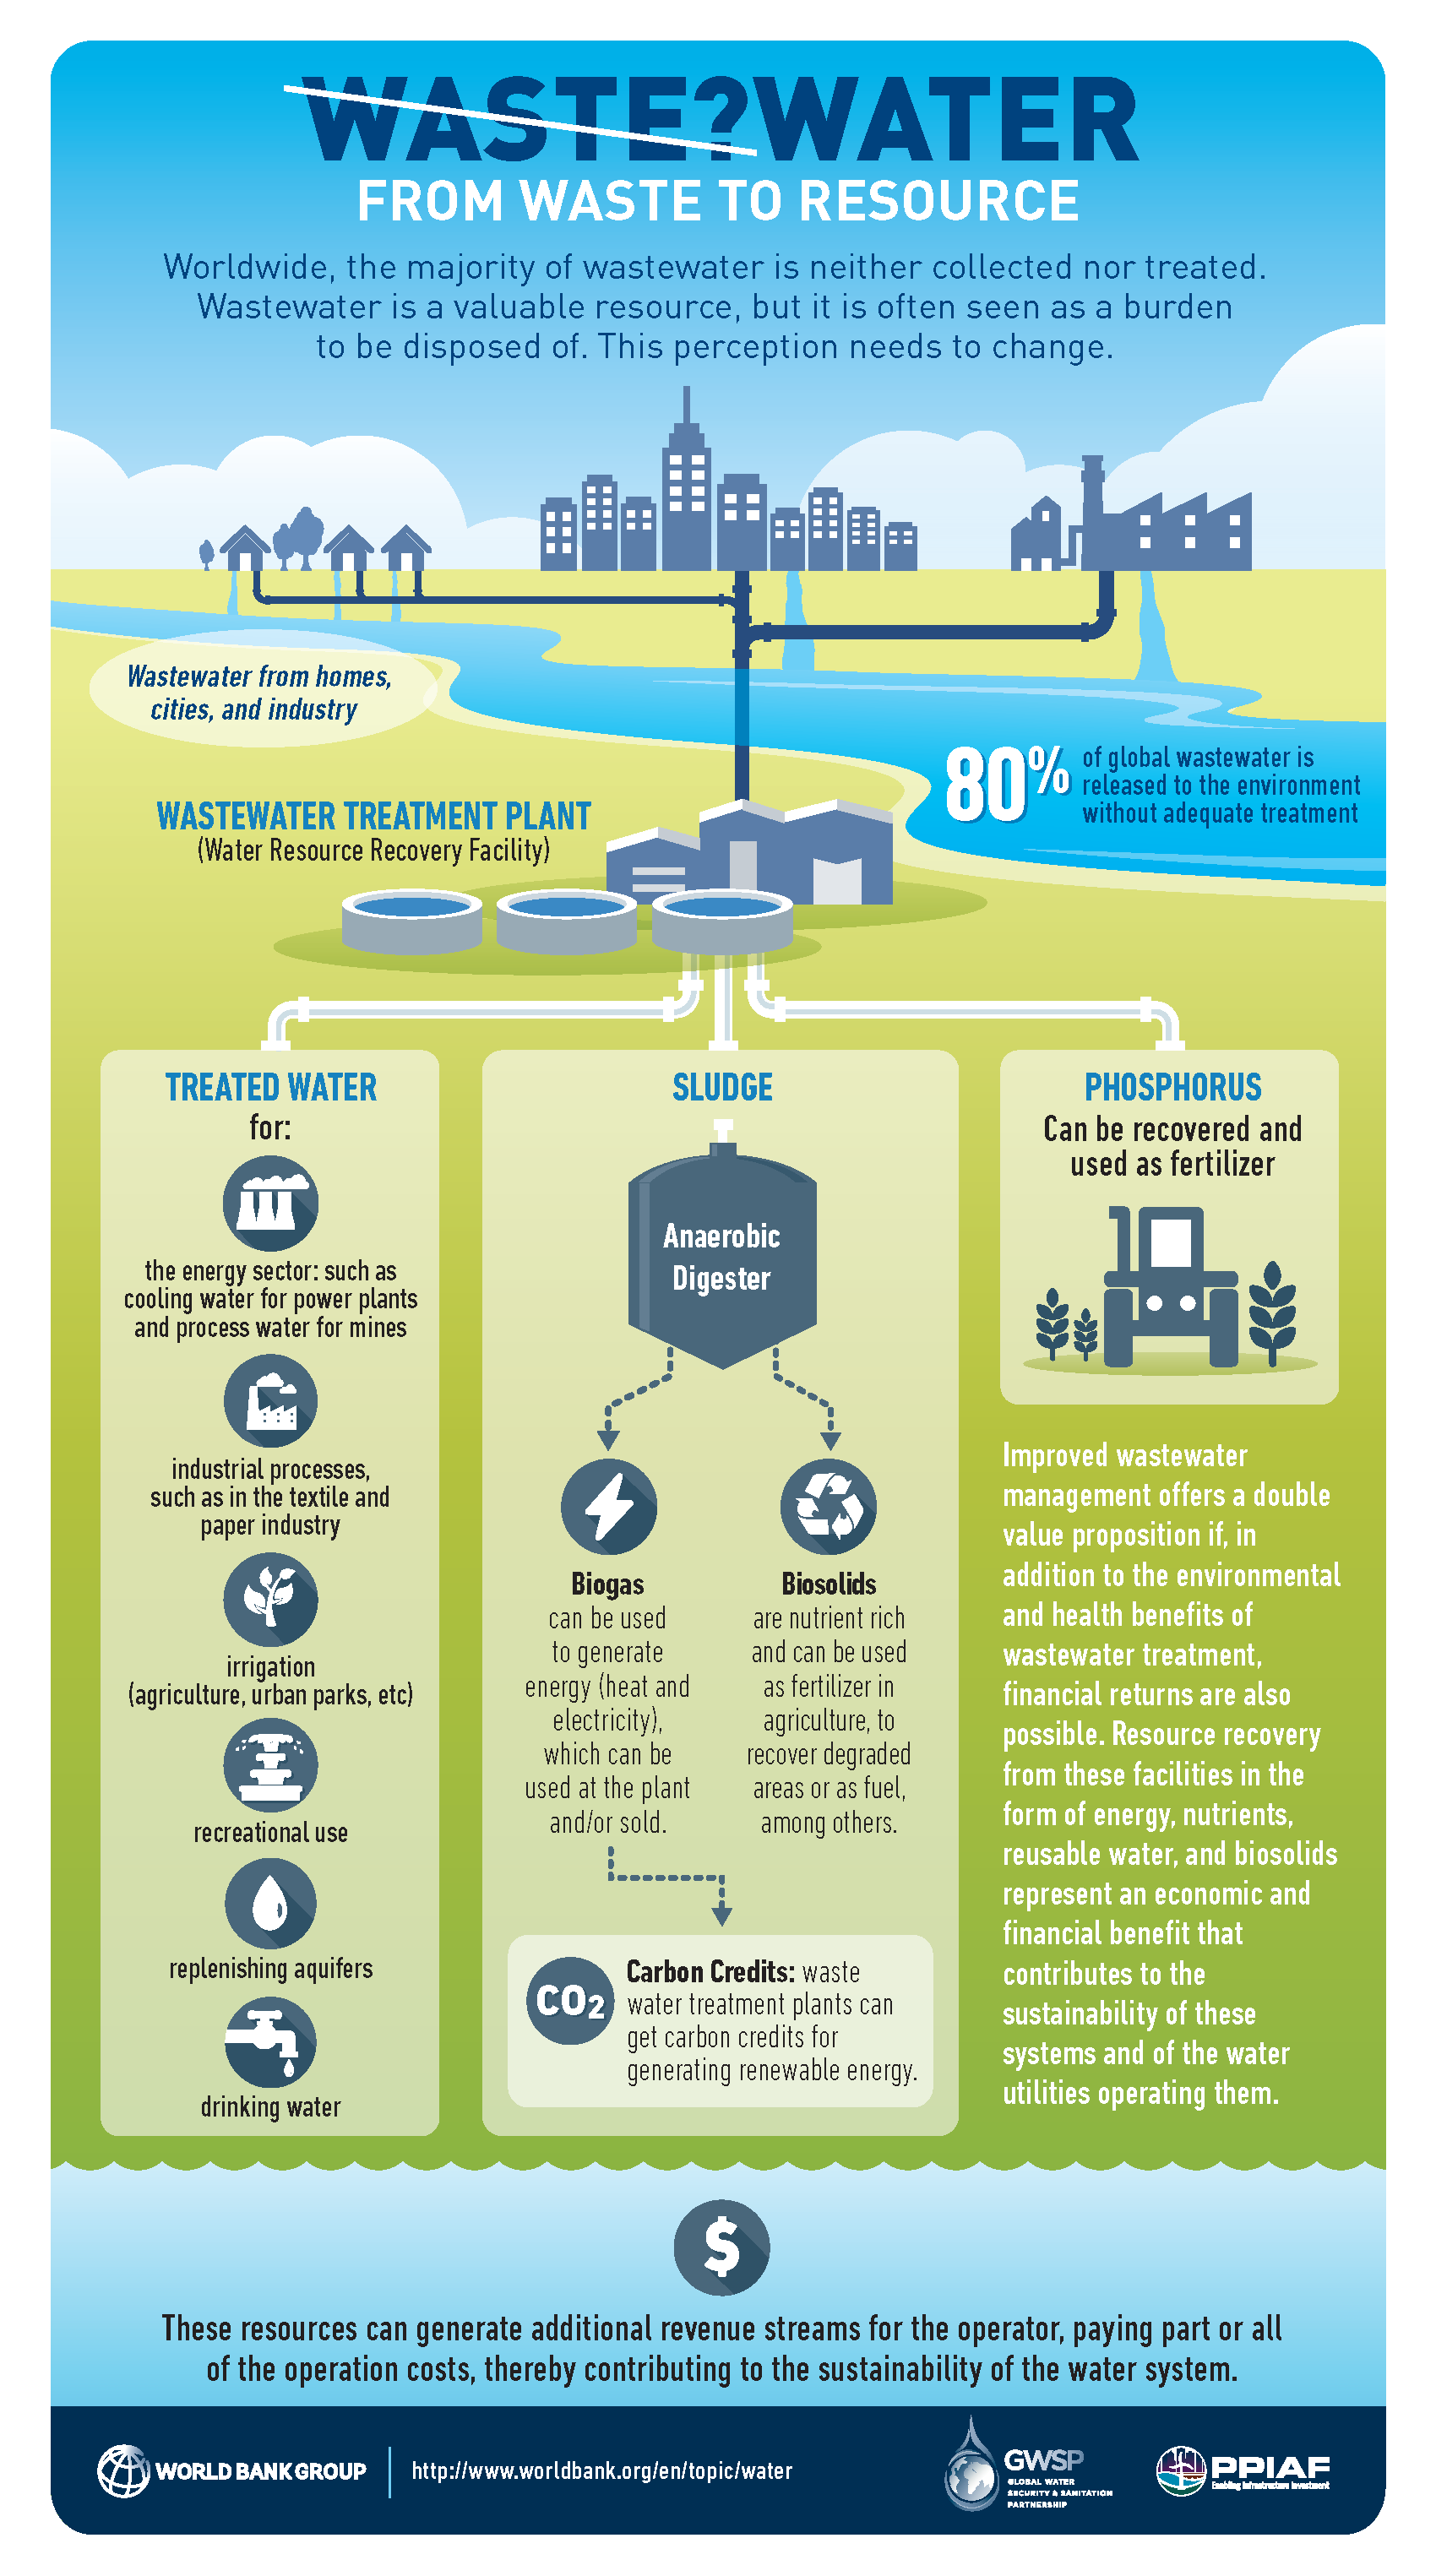
\includegraphics[scale=0.55]{WBWasteWaterResourceinfographic.png}\\
\emph{Source:  Waste to Resource - World Bank}\\
\end{center}








